\documentclass[tikz,border=10pt]{standalone}
\usetikzlibrary{intersections, calc}
\begin{document}
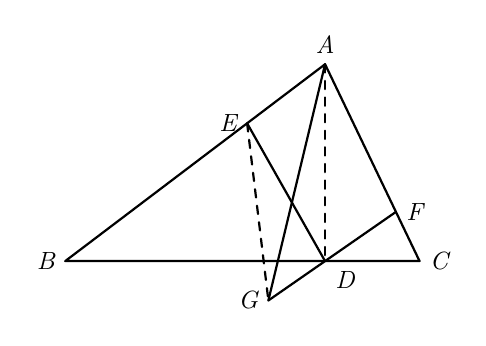
\begin{tikzpicture}[    
line join=round,     
line cap=round,     
thick,     
font=\itshape\small
]    
% 1. 定义三角形顶点    
\coordinate (A) at (3.3, 2.5);    
\coordinate (B) at (0, 0);    
\coordinate (C) at (4.5, 0);
    % 2. 定义内部和外部的关键点    
% D 在 BC 上    
\coordinate (D) at (3.3, 0);    
% E 在 AB 上    
\coordinate (E) at ($(A)!0.3!(B)$);    
% F 在 AC 上    
\coordinate (F) at ($(A)!0.75!(C)$);
    % 3. 定义点 G    
% 观察原图，G 点位于 FD 的延长线上，且处于 AD 射线的左侧    
\coordinate (G) at ($(F)!1.8!(D)$);
    % 4. 绘制线条    
\draw (A) -- (B) -- (C) -- cycle; % 绘制三角形 ABC    
\draw (A) -- (G);                 % 绘制线段 AG    
\draw (E) -- (D);                 % 绘制线段 ED    
\draw (F) -- (G);                 % 绘制线段 FG
\draw[dashed] (E) -- (G); 
\draw[dashed] (A) -- (D); 

    % 5. 标注点名称    
% 根据位置自动调整标签方位    
\node [above] at (A) {A};    
\node [left]  at (B) {B};    
\node [right] at (C) {C};    
\node [below right] at (D) {D};    
\node [left]  at (E) {E};    
\node [right] at (F) {F};    
\node [left] at (G) {G};
\end{tikzpicture}
\end{document}